\documentclass{article}
\usepackage{tikz}
\usetikzlibrary{trees}

\begin{document}
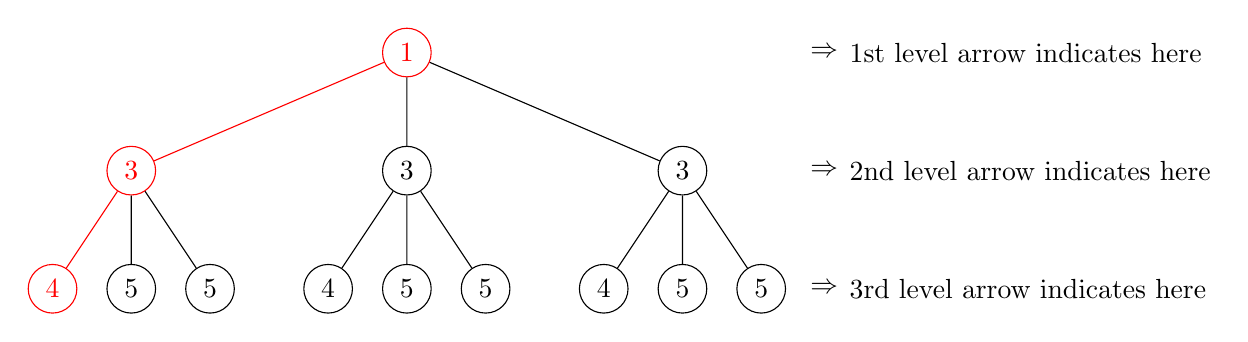
\begin{tikzpicture}[level distance=1.5cm,
level 1/.style={sibling distance=3.5cm},
level 2/.style={sibling distance=1cm}]
\tikzstyle{every node}=[circle,draw]
    \node (Root) [red] {1}
        child [red] {
        node {3}
        child { node {4} }
        child [black] { node {5} }
        child [black] { node {5} }
    }
    child {
        node {3}
        child { node {4} }
        child { node {5} }
        child { node {5} }
    }
    child {
        node {3}
        child { node {4} }
        child { node {5} }
        child { node {5} }
        };
   % Comments to each level
   \begin{scope}[every node/.style={right}]
     \path (Root    -| Root-3-3) ++(5mm,0) node {$\Rightarrow$} ++(5mm,0) node {1st level arrow indicates here};
     \path (Root-1  -| Root-3-3) ++(5mm,0) node {$\Rightarrow$} ++(5mm,0) node {2nd level arrow indicates here};
     \path (Root-1-1-| Root-3-3) ++(5mm,0) node {$\Rightarrow$} ++(5mm,0) node {3rd level arrow indicates here};
   \end{scope}

\end{tikzpicture}
\end{document}